\documentclass[12pt, oneside]{memoir}
\input config.tex
\input glossary.tex

\title{Smart electricity\\
Project report: IT2901}
\author{Beate Baier Biribakken\\
Tor-Håkon Bonsaksen\\
Lars Erik Græsdal-Knutrud\\
Per	Øyvind	Kanestrøm\\
Håvard	Holmboe	Lian\\
Pia	Karlsen	Lindkjølen\\}
\date{Spring 2014}

\makeglossaries
\pagenumbering{gobble}
\begin{document}
%\listoftodos
\maketitle
\newpage
%\lsstyle
\thispagestyle{empty}
\pagenumbering{gobble}

%\titleLL
\clearpage

\renewcommand\contentsname{Contents}
\pagenumbering{Roman}
\tableofcontents*


%\renewcommand\lstlistlistingname{Code snippets}
%\lstlistoflistings

\renewcommand\listfigurename{Figures}
\listoffigures*

\renewcommand\listtablename{Tables}
\listoftables*
	
\cleardoublepage
\pagestyle{headings}
\pagenumbering{arabic}

%Structural:
\todo[inline]{dobbelsjekke om urler er de riktige urlene-> fører til riktig og seriøst nettsted}
\todo[inline]{dobbelsjekke om referansene fungerer som de skal -> at det ikke står et spmtegn der}
\todo[inline]{sjekke at alle illustrasjoner har en caption}
\todo[inline]{sjekke at captionene gir mening. Forklaring bør gjøres i avsnitt som refererer til figuren/tabellen}
\todo[inline]{sjekke at de riktige illustrasjonene er på plass}
\todo[inline]{divide sections into own files}
\todo[inline]{sjekke at sidedelingen er okei, eller om det må legges til at noe begynner på ny linje etc.}
\todo[inline]{Sjekk at alle sections og subsections er riktig og gir mening}
\todo[inline]{Legg til mer om bakgrunnen i beskrivelsen av oppgaven }

%Grammatical:
\todo[inline]{spellcheck}
%\todo[inline]{back end -> back-end}
\todo[inline]{Dobbelsjekke om egennavn er skrevet riktig}
\todo[inline]{check all verbs and formulations for past tense}
\todo[inline]{se over rapporten om vi blir omtalt som noe annet enn the team, our, we; IKKE group, their, they}

\input ch/introduction/introduction.tex
\input ch/prestudy/prestudy.tex
\input ch/projectManagement/projectManagement.tex
\input ch/specification/specification.tex
\input ch/implementation/implementation.tex
\input ch/devProcess/devProcess.tex
\input ch/testing/testing.tex
\input ch/retrospect/retrospect.tex
\input ch/further/further.tex

\glsaddall
\printglossaries
\bibliography{master}

\appendix
\addcontentsline{toc}{chapter}{Appendices}
%\input appendix/usecase/usecase.tex
\input appendix/frozenReq/frozenReq.tex
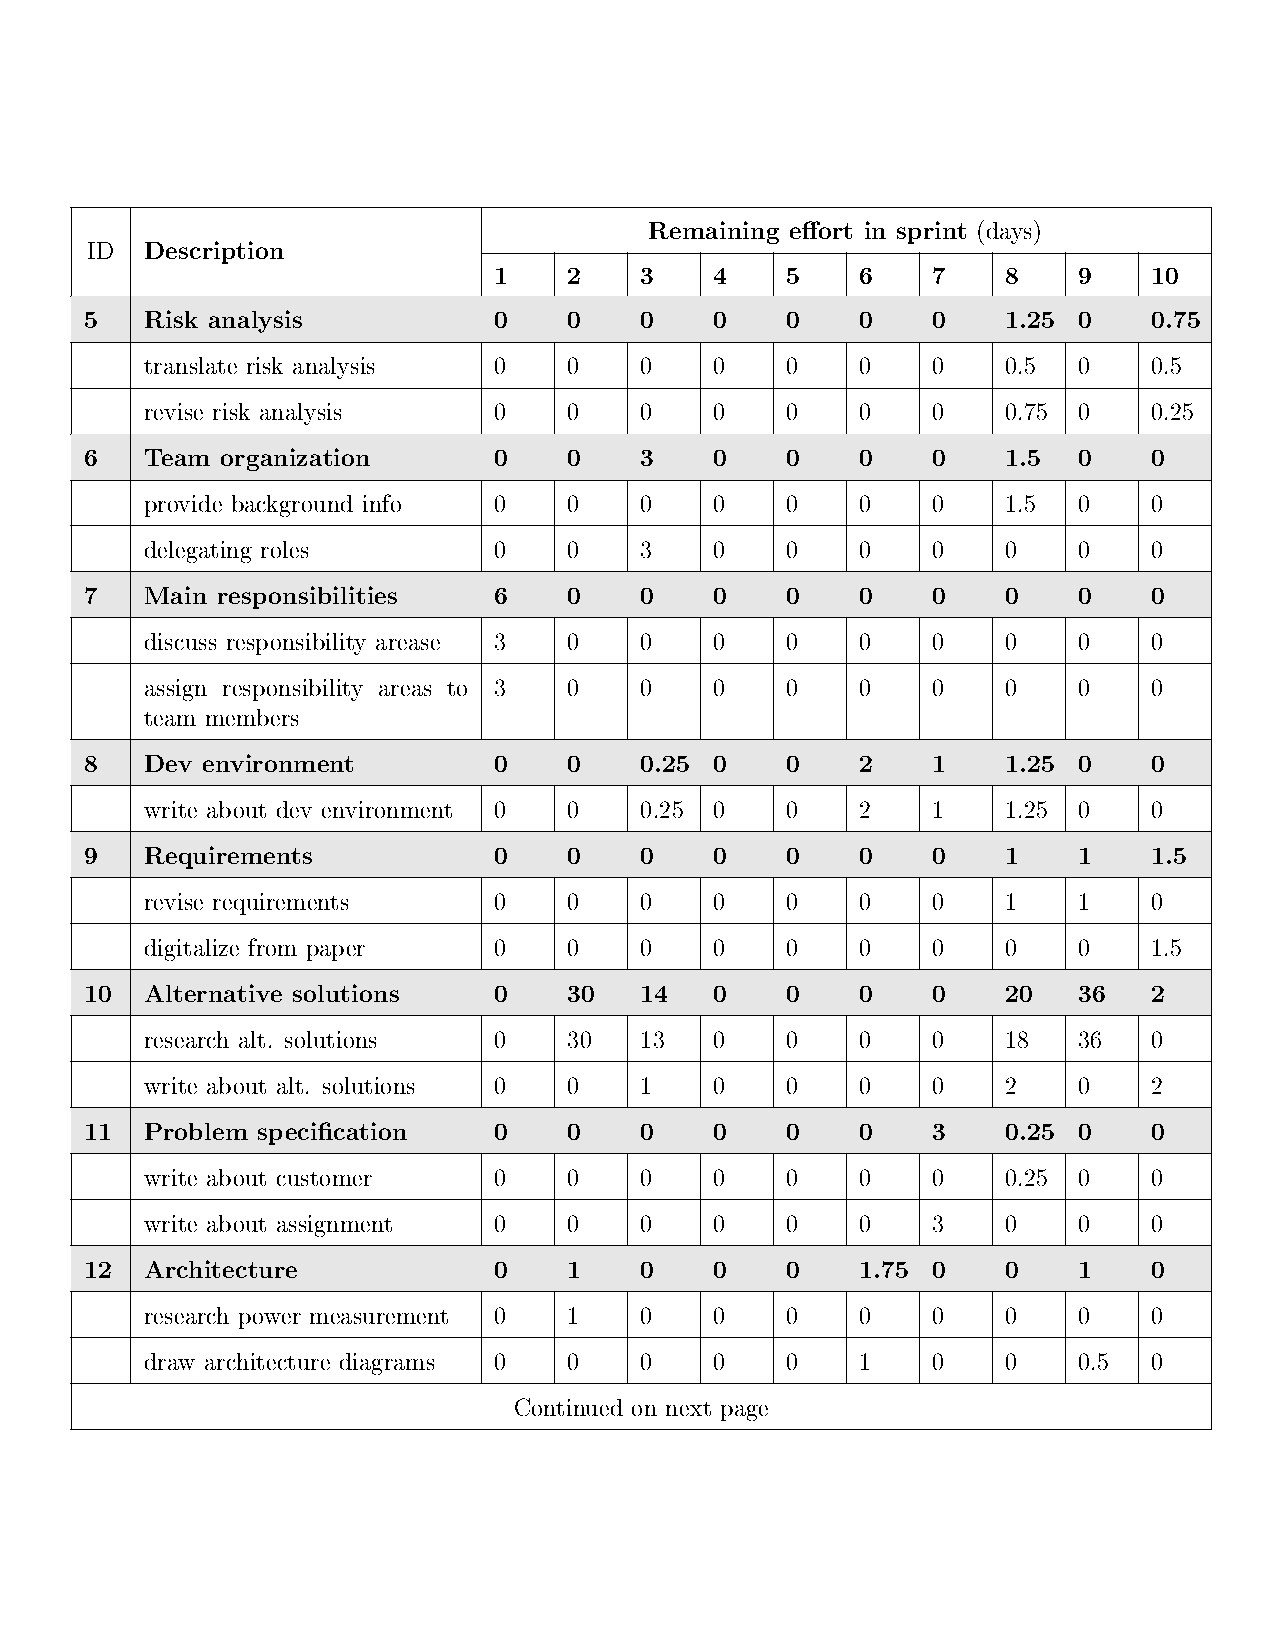
\includepdf[pages=-]{ appendix/backlog/backlogs.pdf}
\input appendix/meetings/meetings.tex
\input appendix/usermanual/usermanual.tex
\input appendix/techDoc/techDoc.tex

\end{document}
